
Due to the detailed planning and devolopment of the GUI elements during the first deliverable the creation of the main operations GUI elements were able to be completed rather swiftly. However there was an initial lag caused by the lack of familiarity with JavaFX and scene builder. After a few hours of familiarization, a FXML closely resembling the protoyped design was created for the main order screen. 

\begin{figure}[ht]
	\centering
	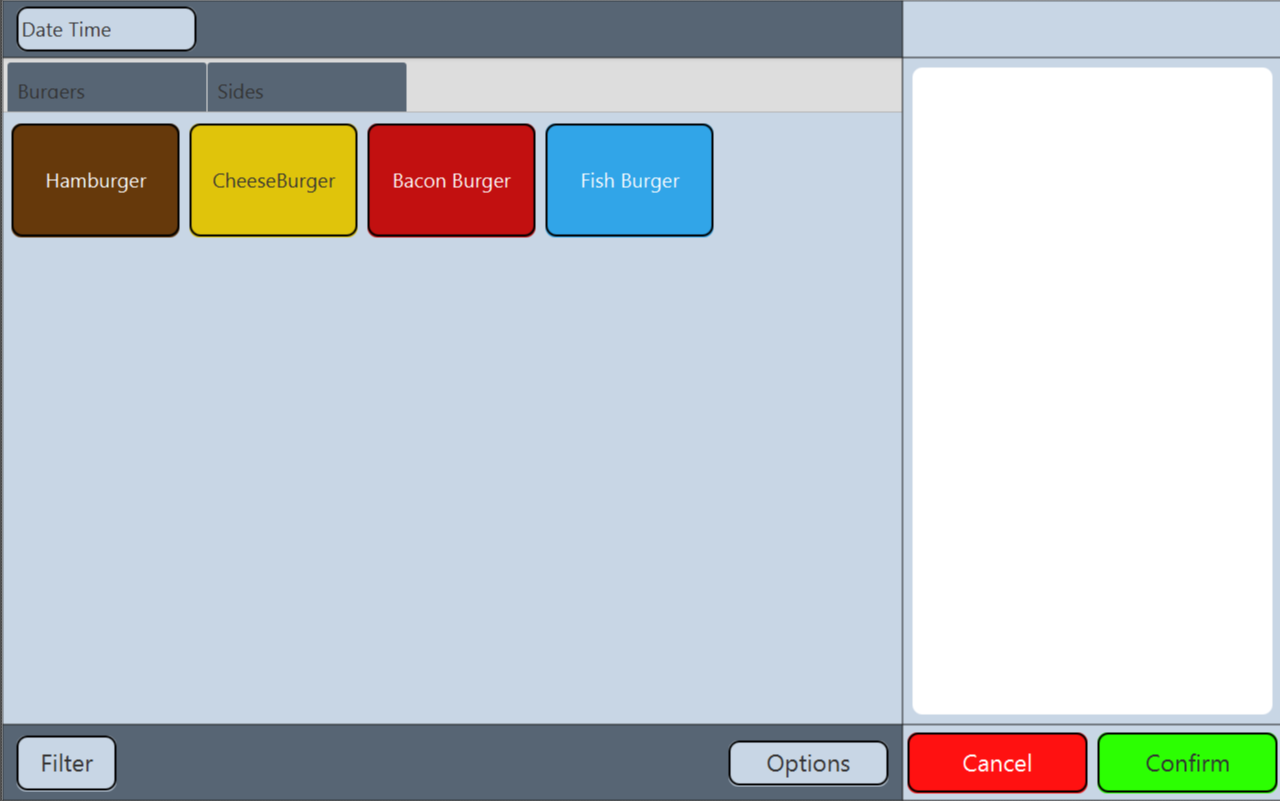
\includegraphics[width=150mm]{images/old_order_screen.png}
	\caption{Initial implimentation of the prototyped design}
	\label{fig:old_order_screen}
\end{figure}

Most of the differences between the first implementation and the prototype (\ref{fig:old_order_screen} and \ref{fig:management_screen_moqueup} respectivly) can be attributed to the differences between the programs used to create them as well as constraints created when implimenting elements with relative alignments or elements that exist within other elements.

The first implimentation of the GUI was effectivly a simple skin of the prototype with buttons that printed their name but no further functionallity. This allowed for a devolopment of basic skills and expereince as well as a platform for further devolopment moving forward. The experience gained from this base was then taken forward and used in the creation of the other UI elements for the operations side whilst refining the main order screen and adding the functionality. The creation of these scenes and their functionallity was significantly easier after getting over the initial learning curve of JavaFX and SceneBuilder.

During this time there was a converstion surrounding the implimentation of the buttons for adding items to orders. Initially the buttons were designed and implimented to all be generated as blank, disabled buttons and then be enabled and filled when needed, however we decided to switch to an approach using buttons that were dynamically created and loaded when the main order screen was loaded in an effort to reduce cluttering of the main order window (QRXX?).

Through out the devolopment of the operations side of the GUI small changes and adjustments were made to the design in an effort to clean and improve elements as they were noticed. An example of this was removing the black outline sorounding each item button. This change gave the main order screen a cleaner appearance, which was part of the driving force for the operational GUI.

The devolopment of the management side GUI was unfortuantly neglected during the planning stages so its devolopment and implimentation became plain and focused on the function when compared to the operations UIs. This caused the initial management screen prototype (see \ref{fig:management_screen_moqueup}) to be paritally overhauled to a more tabular based aproach that focused on presenting information and implimenting functional elements in an efficent and simplified manner.

It is also worth noting that significant efforts towards planning and implimenting the system architecture proved extremely valuable during the implimentation of the functional elements and methods of the GUIs. This allowed for rapid implimentation of features even when under time pressures close to the devlierable deadlines.

Retrospectively the devolopment and implimentation of the GUIs should be considered with a split between the operations and the management sides. This both reflects how the system functions as well as how the GUIs were implimented. 

\begin{figure}[ht]
	\centering
	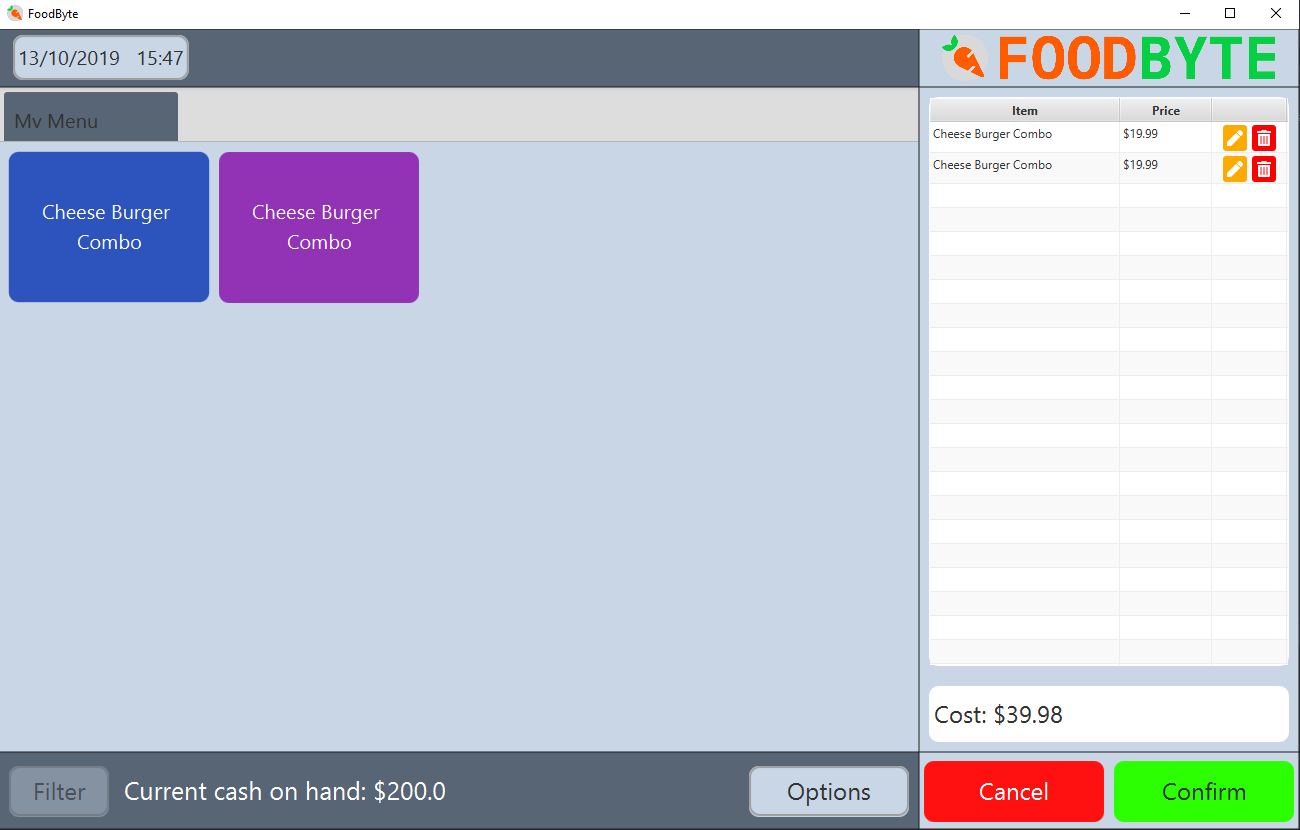
\includegraphics[width=150mm]{images/Final_GUI/main_order_screen.png}
	\caption{Final implimentation of the main order screen}
	\label{fig:final_order_screen}
\end{figure}

The operations side was the major focus during both the planning and the implimentation stages. Because of this there was a very clear plan and style that was carried through strongly into the implimentation stages. This resulted in a final implimentation (\ref{fig:final_order_screen}) that is very similar to the initial design with only a few minor aesthetics changes. The only major change betweeen the prototype and the final implimentation is the change from having pages with next/previous buttons to hold any overflow items for a given menu in the prototype, to a scrolling pane in the final implimentation. This change was made, inspite of our earlier choice to the counter, because it allowed for easier scaling of the interface when the window size was changed whilst not making any major comprimizes towards usability.
All other operations GUI scenes can be found in the apendix.

\begin{figure}[ht]
	\centering
	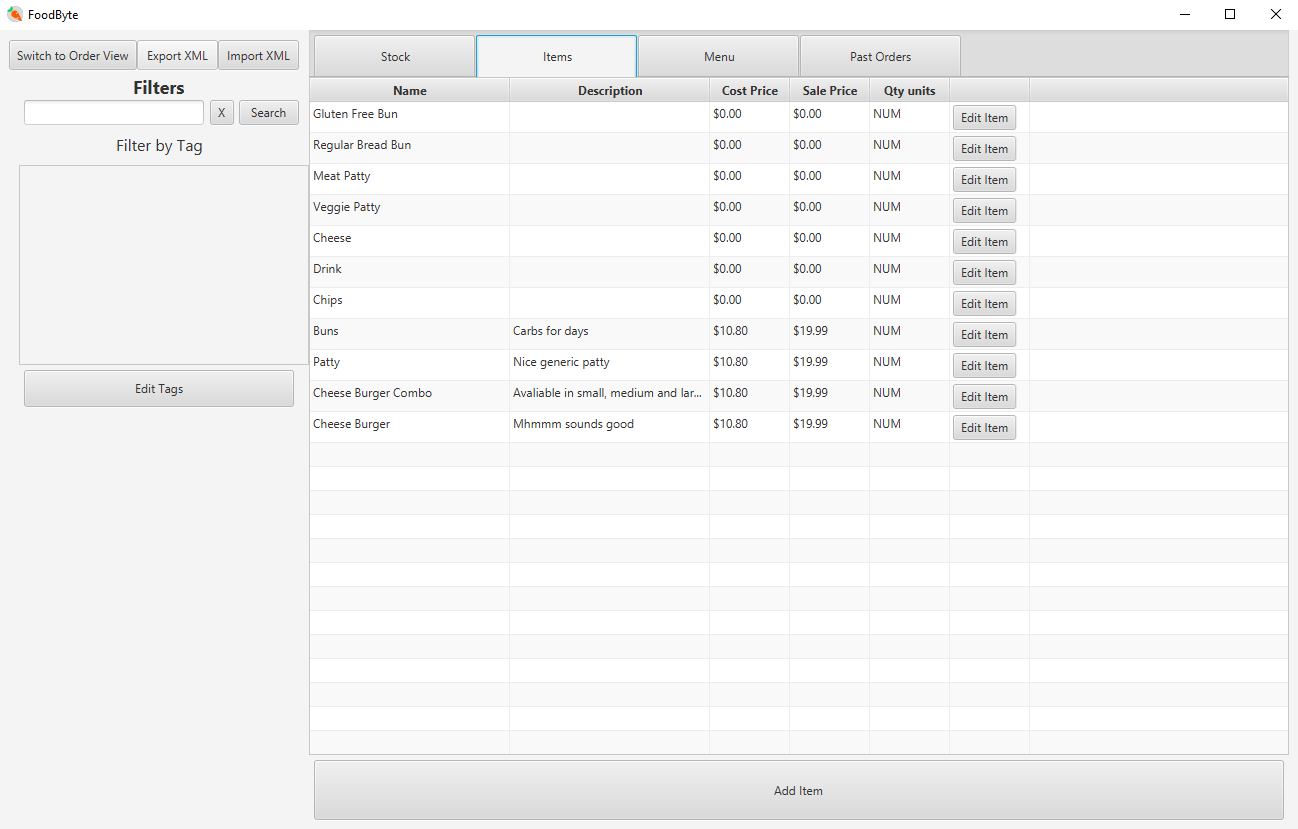
\includegraphics[width=150mm]{images/Final_GUI/item_screen.png}
	\caption{Final implimentation of the item management screen}
	\label{fig:final_item_screen}
\end{figure}

The management side of the GUI was unfortunately neglected during the planning stage and this was also carried through to the implimentation stage. During implimentation the main focus was on creating function and although there was consideration and care towards usability there was little focus towards aesthetics. This has resulted in the manegement side not having the same visual standard as the operations side which is regrettable. The final manegment side UIs (example in \ref{fig:final_item_screen}) ened up implimenting a stripped down tabular focused design. Although the management side is visually lacking when compared to the operations side it was agreed by the devolopment team that, as the operations side will be the main focus of use during deployment, it was more important to have that to a high standard.

When retrospecting the entire aplications UIs as a whole it can be evidanced from the plans and the end result that heavier focus on the operations side has resulted in a application with a very clean and user friendly front end whilst and unfortunately lacklusterr, in comparison, manegment side. If this project were to be further devoloped there is clear room to bring the manegment side up to the same stylazed standard as the operations side and the style used in the operations side should be able to be ported into the manegment side without need for a complete redesign. It is also worth mentioning that there are areas in the options popup in the operations side that would allow for easy insertion of expanded features. On the managment side this could also be acomplished by either adding more tabs to the tab pane or by pulling the tab pane down and useing the row of space above that to impliment more expansions.